% !TEX program = xelatex
\ifdefined\MASTERBOOK\else
\documentclass[UTF8,zihao=-4,oneside,openany]{ctexbook}

% Shared style for the combined handout.  Section files keep standalone
% preambles for now, while the master document uses this single definition.
\usepackage[a4paper,top=20mm,bottom=22mm,left=19mm,right=19mm,headheight=24pt]{geometry}
\usepackage[table]{xcolor}
\usepackage{amsmath,amssymb,mathtools,bm}
\usepackage{siunitx}
\usepackage{booktabs,tabularx,array,multicol}
\usepackage{enumitem}
\usepackage{tikz}
\usetikzlibrary{arrows.meta,positioning,calc,angles,quotes,patterns}
\usepackage[most]{tcolorbox}
\usepackage{fancyhdr}
\usepackage{hyperref}

\definecolor{Ink}{HTML}{202326}
\definecolor{DeepBlue}{HTML}{294E69}
\definecolor{Blue}{HTML}{47687D}
\definecolor{PaleBlue}{HTML}{F3F5F6}
\definecolor{Gold}{HTML}{6E777D}
\definecolor{PaleGold}{HTML}{F6F6F5}
\definecolor{Green}{HTML}{5B6D76}
\definecolor{PaleGreen}{HTML}{F3F5F6}
\definecolor{Alert}{HTML}{666B6F}
\definecolor{PaleAlert}{HTML}{F6F6F6}
\definecolor{RuleGray}{HTML}{D3D7DA}
\definecolor{TextGray}{HTML}{61686D}
\definecolor{SoftGray}{HTML}{F6F6F6}

\color{Ink}
\sisetup{
  per-mode=symbol,
  inter-unit-product=\ensuremath{{}\cdot{}},
  exponent-product=\times
}

\hypersetup{
  colorlinks=true,
  linkcolor=DeepBlue,
  urlcolor=Blue,
  pdfsubject={高中物理竞赛一轮资料重排讲义},
  pdfauthor={物理竞赛一轮资料编写组}
}

\setlength{\parindent}{2em}
\setlength{\parskip}{0.25em}
\setlist{nosep,leftmargin=2em}
\setcounter{secnumdepth}{3}
\setcounter{tocdepth}{2}
\numberwithin{equation}{section}
\counterwithin{table}{section}
\allowdisplaybreaks[2]
\emergencystretch=2em

\ctexset{
  chapter={
    format=\raggedright\LARGE\bfseries\color{Ink},
    titleformat=\LARGE\bfseries\color{Ink},
    beforeskip=0pt,
    afterskip=18pt
  },
  section={
    format=\Large\bfseries\color{DeepBlue},
    beforeskip=1.8ex,
    afterskip=1.0ex
  },
  subsection={
    format=\large\bfseries\color{Ink},
    beforeskip=1.5ex,
    afterskip=0.8ex
  },
  subsubsection={format=\normalsize\bfseries\color{Ink}}
}

\pagestyle{fancy}
\fancyhf{}
\fancyhead[L]{\small\color{TextGray}高中物理竞赛一轮讲义}
\fancyhead[R]{\small\color{TextGray}第一章\quad 数学与物理工具}
\fancyfoot[C]{\small\color{TextGray}\thepage}
\renewcommand{\headrulewidth}{0.4pt}
\renewcommand{\headrule}{\hbox to\headwidth{\color{RuleGray}\leaders\hrule height \headrulewidth\hfill}}

\newcommand{\dimens}[1]{\operatorname{dim}\!\left(#1\right)}
\newcommand{\dd}{\mathop{}\!\mathrm{d}}
\newcommand{\vect}[1]{\bm{#1}}
\newcommand{\uvec}[1]{\hat{\vect{#1}}}
\newcommand{\e}{\mathrm e}
\newcommand{\order}[1]{\mathcal O\!\left(#1\right)}
\DeclareMathOperator{\proj}{proj}
\newcommand{\examplesource}[1]{%
  \par{\small\color{TextGray}题源：#1}\par
}

\newtcolorbox{goalbox}{
  enhanced,breakable,
  colback=PaleBlue,colframe=Blue,
  boxrule=0.7pt,arc=2mm,
  title={本节目标},fonttitle=\bfseries,
  coltitle=DeepBlue,
  attach boxed title to top left={xshift=5mm,yshift=-2mm},
  boxed title style={colback=white,colframe=Blue,boxrule=0.7pt,arc=1.5mm}
}

\newtcolorbox{sourcebox}{
  enhanced,breakable,
  colback=SoftGray,colframe=RuleGray,
  boxrule=0.5pt,arc=0mm,
  title={题源说明},fonttitle=\bfseries,
  coltitle=Ink,colbacktitle=SoftGray,
  borderline west={1.2pt}{0pt}{TextGray}
}

\newtcolorbox[auto counter,number within=section]{examplebox}[2][]{
  enhanced,breakable,
  colback=white,colframe=RuleGray,
  boxrule=0.5pt,arc=0mm,
  title={例题~\thetcbcounter\quad #2},fonttitle=\bfseries,
  coltitle=Ink,colbacktitle=PaleBlue,
  borderline west={1.4pt}{0pt}{DeepBlue},
  #1
}

\newtcolorbox{methodbox}[1]{
  enhanced,breakable,
  colback=PaleBlue,colframe=RuleGray,
  boxrule=0.5pt,arc=0mm,
  title={方法：#1},fonttitle=\bfseries,
  coltitle=Ink,colbacktitle=PaleBlue,
  borderline west={1.2pt}{0pt}{DeepBlue}
}

\newtcolorbox{warningbox}[1]{
  enhanced,breakable,
  colback=SoftGray,colframe=RuleGray,
  boxrule=0.5pt,arc=0mm,
  title={易错提醒：#1},fonttitle=\bfseries,
  coltitle=Ink,colbacktitle=SoftGray,
  borderline west={1.2pt}{0pt}{TextGray}
}

\newtcolorbox{extensionbox}[1]{
  enhanced,breakable,
  colback=PaleGold,colframe=Gold,
  boxrule=0.5pt,arc=0mm,
  title={拓展：#1},fonttitle=\bfseries,
  coltitle=Ink,colbacktitle=PaleGold,
  borderline west={1.2pt}{0pt}{DeepBlue}
}

\newtcolorbox{summarybox}{
  enhanced,breakable,
  colback=PaleBlue,colframe=DeepBlue,
  boxrule=0.9pt,arc=1.5mm,
  title={本节小结},fonttitle=\bfseries,
  coltitle=white,colbacktitle=DeepBlue
}

\newtcolorbox{exercisebox}[1]{
  enhanced,breakable,
  colback=white,colframe=RuleGray,
  boxrule=0.7pt,arc=1.5mm,
  title={#1},fonttitle=\bfseries,
  coltitle=DeepBlue,colbacktitle=PaleBlue
}

\tikzset{
  vector/.style={-{Latex[length=2.5mm]},very thick,draw=DeepBlue},
  component/.style={-{Latex[length=2.2mm]},thick,draw=TextGray},
  axis/.style={-{Latex[length=2mm]},thin,draw=TextGray},
  guide/.style={densely dashed,draw=TextGray},
  curve/.style={very thick,draw=DeepBlue},
  tangent/.style={thick,draw=TextGray},
  secant/.style={thick,draw=DeepBlue}
}


\hypersetup{
  pdftitle={高中物理竞赛一轮讲义样章：微分方程、初始条件与典型变化规律}
}

\begin{document}

\pagenumbering{arabic}
\setcounter{page}{1}
\setcounter{chapter}{0}
\chapter{数学与物理工具}
\setcounter{section}{3}
\fi
\ifdefined\MASTERBOOK\clearpage\fi
\section{微分方程、初始条件与典型变化规律}

物理定律往往先给出“系统怎样变化”，而不是直接给出“系统在任意时刻是什么状态”。
例如牛顿第二定律把加速度与受力联系起来，放射性衰变规律把原子数的变化率与当前原子数
联系起来。这类含有未知函数及其导数的关系称为微分方程。求解微分方程，就是从局部的
变化规律和初始状态出发，恢复系统的完整演化过程。

本节承接上一节的导数、积分与微元思想，重点讨论竞赛中最常见的一阶可分离变量方程，
并说明怎样利用链式法则处理位置相关的二阶动力学问题。每个结果都将检查初值、量纲、
短时极限和长时行为，使方程的解重新回到清楚的物理图像中。

\begin{sourcebox}
本节例题 1.4.1--1.4.5 改编自学而思
《19春假兴趣2—微积分在物理学中的应用》例 1.23--1.27（原 PDF 第 18--20 页）。
保留原题的物理模型和已知条件，统一了符号、正方向与单位，并补写完整推导、结果检验和
模型解释。新增的图示均由 TikZ 绘制。
\end{sourcebox}

\subsection{从物理定律到微分方程}

若未知物理量是 $y(t)$，一个最常见的一阶微分方程可写成
\begin{equation}
  \frac{\dd y}{\dd t}=F(t,y).
  \label{eq:first-order-ode}
\end{equation}
方程右侧给出状态 $y$ 在时刻 $t$ 的瞬时变化率。仅有方程通常还不能确定唯一过程，
还需要一个初始条件
\begin{equation}
  y(t_0)=y_0.
  \label{eq:first-order-initial-condition}
\end{equation}
例如 $\dd y/\dd t=-ky$ 的解包含任意常数 $C$：$y=C\e^{-kt}$；只有再给出
$y(0)=y_0$，才能确定 $C=y_0$。

质点的一维动力学通常给出二阶方程
\begin{equation}
  m\frac{\dd^2x}{\dd t^2}=F\!\left(t,x,\frac{\dd x}{\dd t}\right).
  \label{eq:second-order-dynamics}
\end{equation}
二阶方程一般需要两个彼此独立的初始条件，例如 $x(t_0)=x_0$ 和
$v(t_0)=v_0$。位置说明质点从哪里出发，速度说明它以怎样的状态出发；缺少其中任何
一个，都可能对应一族不同的运动。

\begin{methodbox}{建模—初值—求解—检验}
\begin{enumerate}[label=\arabic*.]
  \item 规定坐标轴、正方向和未知函数，先写有符号的物理定律；
  \item 把初始时刻与初始状态单独列出，并判断条件数是否与方程阶数匹配；
  \item 选择变量分离、换元或降阶方法，尽量使用带上下限的定积分；
  \item 检查初值、量纲、特殊极限，并把结果代回原微分方程。
\end{enumerate}
\end{methodbox}

\subsection{一阶可分离变量方程}

若一阶方程能够整理成
\begin{equation}
  \frac{\dd y}{\dd t}=g(t)h(y),
  \label{eq:separable-ode}
\end{equation}
就在 $h(y)\ne0$ 的区间内把含 $y$ 与含 $t$ 的量分到两侧：
\[
  \frac{\dd y}{h(y)}=g(t)\,\dd t.
\]
把初始条件直接写进积分限，可得
\begin{equation}
  \int_{y_0}^{y(t)}\frac{\dd u}{h(u)}
  =\int_{t_0}^{t}g(s)\,\dd s.
  \label{eq:separable-integral-form}
\end{equation}
这里 $u,s$ 是积分中的哑变量，不应与积分上限 $y(t),t$ 混用。式
\eqref{eq:separable-integral-form} 已经自动包含初始条件，因此不需要再补一个来源不明的
积分常数。

\begin{warningbox}{除以未知量可能丢失平衡解}
若 $h(y_*)=0$，则常值函数 $y(t)=y_*$ 本身可能就是原方程的解。直接除以 $h(y)$
会把这一解排除，所以变量分离之前必须先检查被除量能否为零。
\end{warningbox}

\begin{examplebox}{线性阻力下的减速运动}
\examplesource{学而思《19春假兴趣2—微积分在物理学中的应用》例 1.23，第 18 页；解答重写。}
质量为 $m$ 的质点沿 $x$ 轴正方向运动，受到与速度成正比的阻力
$f=-\alpha v$。已知 $t=0$ 时 $v=v_0>0$、$x=0$。求 $v(t)$、$x(t)$
以及 $v(x)$。

\tcblower
在质点尚未改变运动方向时，牛顿第二定律为
\begin{equation}
  m\frac{\dd v}{\dd t}=-\alpha v.
  \label{eq:linear-drag-ode}
\end{equation}
由 $[\alpha]=\mathsf M\mathsf T^{-1}$ 可定义特征时间
\begin{equation}
  \tau=\frac{m}{\alpha}.
  \label{eq:linear-drag-timescale}
\end{equation}
对式 \eqref{eq:linear-drag-ode} 分离变量，并把 $v(0)=v_0$ 写入积分限：
\begin{align*}
  \int_{v_0}^{v(t)}\frac{\dd u}{u}
  &=-\frac1\tau\int_0^t\dd s,\\
  \ln\frac{v(t)}{v_0}&=-\frac{t}{\tau}.
\end{align*}
因此
\begin{equation}
  v(t)=v_0\e^{-t/\tau}.
  \label{eq:linear-drag-velocity}
\end{equation}
再由 $\dd x/\dd t=v(t)$ 积分：
\begin{align*}
  x(t)
  &=\int_0^t v_0\e^{-s/\tau}\,\dd s\\
  &=v_0\tau\left(1-\e^{-t/\tau}\right).
\end{align*}
当 $t\to\infty$ 时，速度无限趋近于零，前进距离趋近有限值
\begin{equation}
  x_\infty=v_0\tau=\frac{mv_0}{\alpha}.
  \label{eq:linear-drag-distance}
\end{equation}

为求 $v(x)$，利用链式法则 $\dd v/\dd t=v\,\dd v/\dd x$。在 $v>0$ 的阶段，
\[
  mv\frac{\dd v}{\dd x}=-\alpha v
  \quad\Longrightarrow\quad
  \frac{\dd v}{\dd x}=-\frac{\alpha}{m}=-\frac1\tau.
\]
结合 $v(0)=v_0$，得到
\begin{equation}
  v(x)=v_0-\frac{x}{\tau}
  =v_0\left(1-\frac{x}{x_\infty}\right),
  \qquad 0\le x<x_\infty.
  \label{eq:linear-drag-vx}
\end{equation}
代入 $t=0$ 可得 $v=v_0,x=0$；对式 \eqref{eq:linear-drag-velocity} 求导，
又有 $m\dot v=-\alpha v$，初值和原方程都得到满足。
\end{examplebox}

\subsection{平衡值、终端速度与换元}

方程右侧为零的状态称为平衡值。若系统偏离这一状态后会逐渐返回，它就是稳定平衡值。
对于含有恒定驱动力和线性阻力的方程
\begin{equation}
  m\frac{\dd v}{\dd t}=F_0-\alpha v,
  \label{eq:driven-linear-drag}
\end{equation}
令右侧为零，立即得到平衡速度 $v_*=F_0/\alpha$。换元
$u=v-v_*$，便把式 \eqref{eq:driven-linear-drag} 化成
$m\dot u=-\alpha u$。因此，复杂之处不是重新求一种解，而是先找出应该围绕哪个平衡值
研究偏差。

\begin{examplebox}{重力与线性阻力共同作用的下落}
\examplesource{学而思《19春假兴趣2—微积分在物理学中的应用》例 1.24，第 18--19 页；解答重写。}
质量为 $m$ 的物体从静止开始竖直下落，同时受到与速度成正比的阻力
$f=-\alpha v$。取竖直向下为正方向，求速度 $v(t)$，并进一步求位移和加速度。

\tcblower
重力沿正方向，阻力在 $v\ge0$ 时沿负方向，所以
\begin{equation}
  m\frac{\dd v}{\dd t}=mg-\alpha v.
  \label{eq:falling-linear-drag-ode}
\end{equation}
定义
\begin{equation}
  v_{\mathrm T}=\frac{mg}{\alpha},
  \qquad
  \tau=\frac{m}{\alpha},
  \label{eq:terminal-speed-and-time}
\end{equation}
其中 $v_{\mathrm T}$ 是令合力为零得到的终端速度。原方程变为
\[
  \frac{\dd v}{\dd t}=\frac{v_{\mathrm T}-v}{\tau}.
\]
由初值 $v(0)=0$ 分离变量：
\begin{align*}
  \int_0^{v(t)}\frac{\dd u}{v_{\mathrm T}-u}
  &=\frac1\tau\int_0^t\dd s,\\
  \ln\frac{v_{\mathrm T}}{v_{\mathrm T}-v(t)}
  &=\frac{t}{\tau}.
\end{align*}
解得
\begin{equation}
  v(t)=v_{\mathrm T}\left(1-\e^{-t/\tau}\right).
  \label{eq:falling-linear-drag-velocity}
\end{equation}
继续积分速度，并取 $x(0)=0$：
\begin{align}
  x(t)
  &=\int_0^t v_{\mathrm T}\left(1-\e^{-s/\tau}\right)\dd s\notag\\
  &=v_{\mathrm T}\left[t-\tau\left(1-\e^{-t/\tau}\right)\right].
  \label{eq:falling-linear-drag-position}
\end{align}
对速度求导得到
\begin{equation}
  a(t)=g\e^{-t/\tau}.
  \label{eq:falling-linear-drag-acceleration}
\end{equation}
短时间 $t\ll\tau$ 时，$\e^{-t/\tau}\approx1-t/\tau$，于是
$v\approx gt$、$x\approx\frac12gt^2$，恢复自由落体；长时间 $t\gg\tau$ 时，
$v\to v_{\mathrm T}$、$a\to0$。两个极限都符合受力图像。
\end{examplebox}

\subsection{平方阻力与代数衰减}

阻力模型取决于速度范围与流动状态。线性阻力给出指数衰减；若阻力大小与 $v^2$
成正比，速度的衰减规律会发生本质变化。

\begin{examplebox}{平方阻力下的减速运动}
\examplesource{学而思《19春假兴趣2—微积分在物理学中的应用》例 1.25，第 19 页；解答重写。}
质量为 $m$ 的质点从 $x=0$ 处以初速度 $v_0>0$ 出发，受到平方阻力
$f=-\beta v^2$。求速度随时间的变化规律，并求 $x(t)$。

\tcblower
牛顿第二定律为
\begin{equation}
  m\frac{\dd v}{\dd t}=-\beta v^2.
  \label{eq:quadratic-drag-ode}
\end{equation}
分离变量后积分：
\begin{align*}
  \int_{v_0}^{v(t)}\frac{\dd u}{u^2}
  &=-\frac{\beta}{m}\int_0^t\dd s,\\
  -\frac1{v(t)}+\frac1{v_0}
  &=-\frac{\beta}{m}t.
\end{align*}
整理得
\begin{equation}
  v(t)=\frac{v_0}{1+t/t_2},
  \qquad
  t_2=\frac{m}{\beta v_0}.
  \label{eq:quadratic-drag-velocity}
\end{equation}
由 $[\beta]=\mathsf M\mathsf L^{-1}$ 可知 $t_2$ 的确具有时间量纲；并且
$v(t_2)=v_0/2$，所以 $t_2$ 正是速度降到一半所需的时间。

位置由速度积分得到：
\begin{align}
  x(t)
  &=\int_0^t\frac{v_0}{1+s/t_2}\,\dd s\notag\\
  &=v_0t_2\ln\left(1+\frac{t}{t_2}\right)
  =\frac{m}{\beta}\ln\left(1+\frac{t}{t_2}\right).
  \label{eq:quadratic-drag-position}
\end{align}
平方阻力下 $v\sim t^{-1}$，衰减慢于指数函数，因此 $x(t)$ 随时间对数增长，
在这个理想模型中没有有限的总前进距离。
\end{examplebox}

令横轴为无量纲时间 $s$，纵轴为归一化速度，可以直接比较两种衰减：
\begin{center}
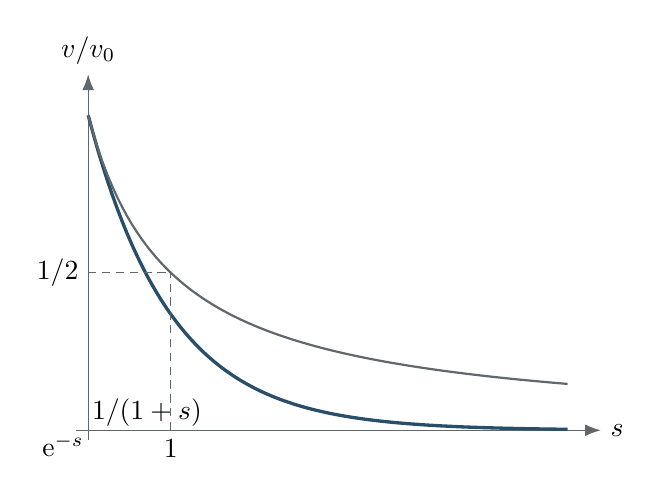
\begin{tikzpicture}[x=1.05cm,y=4.0cm]
  \draw[axis] (-0.15,0)--(6.2,0) node[right] {$s$};
  \draw[axis] (0,-0.03)--(0,1.13) node[above] {$v/v_0$};
  \draw[curve,domain=0:5.8,samples=100]
    plot (\x,{exp(-\x)}) node[pos=0.42,below left,fill=white,inner sep=1pt]
    {$\e^{-s}$};
  \draw[tangent,domain=0:5.8,samples=100]
    plot (\x,{1/(1+\x)}) node[pos=0.68,above right,fill=white,inner sep=1pt]
    {$1/(1+s)$};
  \draw[guide] (0,0.5)--(1,0.5);
  \draw[guide] (1,0)--(1,0.5);
  \node[below] at (1,0) {$1$};
  \node[left] at (0,0.5) {$1/2$};
\end{tikzpicture}
\end{center}
指数曲线在 $s=1$ 时已降为 $\e^{-1}v_0$，平方阻力对应的代数曲线则降为
$v_0/2$。图像差异来自微分方程中速度幂次的不同，而不是由初始条件造成。

\subsection{指数规律与半衰期}

只要某个量的减少速率正比于它当前的大小，就会出现指数规律。线性阻力中的速度偏差、
电容放电中的电荷量以及放射性原子数都属于这一结构。

\begin{examplebox}{放射性衰变与半衰期}
\examplesource{学而思《19春假兴趣2—微积分在物理学中的应用》例 1.27，第 19--20 页；解答重写。}
对含有大量原子的样品，把尚未衰变原子数的平均值作连续近似，记为 $N(t)$。在极短时间内，
平均衰变数正比于当前未衰变原子数，因而
\[
  \frac{\dd N}{\dd t}=-\lambda N,
\]
其中 $\lambda>0$ 为衰变常数。若 $N(0)=N_0$，求 $N(t)$，并给出半衰期
$T_{1/2}$ 与 $\lambda$ 的关系。

\tcblower
负号表示未衰变原子数随时间减少。分离变量并使用初值：
\begin{align*}
  \int_{N_0}^{N(t)}\frac{\dd u}{u}
  &=-\lambda\int_0^t\dd s,\\
  \ln\frac{N(t)}{N_0}&=-\lambda t.
\end{align*}
所以
\begin{equation}
  N(t)=N_0\e^{-\lambda t}.
  \label{eq:radioactive-decay}
\end{equation}
半衰期由 $N(T_{1/2})=N_0/2$ 定义：
\[
  \frac12=\e^{-\lambda T_{1/2}}.
\]
两边取自然对数，得到
\begin{equation}
  T_{1/2}=\frac{\ln2}{\lambda}.
  \label{eq:half-life}
\end{equation}
经过 $n$ 个半衰期后，$N=N_0/2^n$。单位时间内的平均衰变数在连续模型中写成活度
\begin{equation}
  A(t)=-\frac{\dd N}{\dd t}=\lambda N_0\e^{-\lambda t}.
  \label{eq:radioactive-activity}
\end{equation}
由于 $\lambda t$ 必须无量纲，$[\lambda]=\mathsf T^{-1}$，与式
\eqref{eq:half-life} 的量纲一致。
\end{examplebox}

\subsection{位置相关力与二阶方程降阶}

若一维运动的加速度只依赖位置，方程为 $\ddot x=a(x)$。利用
\begin{equation}
  \ddot x=\frac{\dd v}{\dd t}
  =\frac{\dd v}{\dd x}\frac{\dd x}{\dd t}
  =v\frac{\dd v}{\dd x},
  \label{eq:ode-order-reduction}
\end{equation}
就能把关于时间的二阶方程降为关于位置的一阶方程。积分后得到速度与位置的关系，
再由 $\dd t=\dd x/v(x)$ 求运动时间。

\begin{examplebox}{万有引力作用下的径向下落}
\examplesource{学而思《19春假兴趣2—微积分在物理学中的应用》例 1.26，第 19 页；解答重写。}
质量为 $M$ 的物体 $A$ 固定在原点。质量 $m\ll M$ 的质点从距离 $A$ 为 $r_0$
的位置由静止开始径向下落。把两物体视为质点，求相撞时间。

\tcblower
取径向向外为 $r$ 的正方向。质点下落时 $r$ 减小，运动方程为
\begin{equation}
  \ddot r=-\frac{GM}{r^2},
  \qquad r(0)=r_0,\quad \dot r(0)=0.
  \label{eq:radial-fall-ode}
\end{equation}

\begin{center}
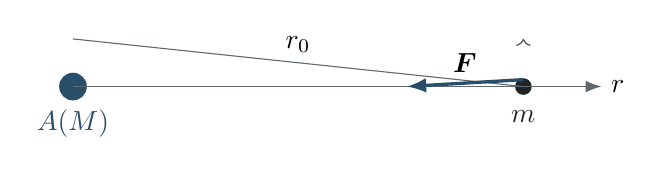
\begin{tikzpicture}[x=1.1cm,y=1.1cm]
  \coordinate (A) at (0,0);
  \coordinate (P) at (5.2,0);
  \fill[DeepBlue] (A) circle (5pt) node[below=5pt] {$A(M)$};
  \fill[Ink] (P) circle (3pt) node[below=5pt] {$m$};
  \draw[axis] (A)--(6.1,0) node[right] {$r$};
  \draw[<->,draw=TextGray] (A)+(0,0.55)--(P)+(0,0.55)
    node[midway,above] {$r_0$};
  \draw[vector] (P)+(0,0.08)--++(-1.35,0) node[midway,above] {$\vect F$};
\end{tikzpicture}
\end{center}

用 $\ddot r=\dot r\,\dd\dot r/\dd r$ 降阶：
\[
  \dot r\frac{\dd\dot r}{\dd r}=-\frac{GM}{r^2}.
\]
从初态 $(r_0,0)$ 积分到 $(r,\dot r)$：
\begin{align*}
  \int_0^{\dot r}\!u\,\dd u
  &=-GM\int_{r_0}^{r}\frac{\dd s}{s^2},\\
  \frac12\dot r^2
  &=GM\left(\frac1r-\frac1{r_0}\right).
\end{align*}
下落时 $\dot r<0$，所以向内速率 $u_r=-\dot r$ 为
\begin{equation}
  u_r(r)=\sqrt{2GM\left(\frac1r-\frac1{r_0}\right)}.
  \label{eq:radial-fall-speed}
\end{equation}
相撞时间是从 $r_0$ 减小到 $0$ 所需的时间：
\begin{equation}
  t_{\mathrm c}=\int_0^{r_0}
  \frac{\dd r}{\sqrt{2GM(1/r-1/r_0)}}.
  \label{eq:radial-fall-time-integral}
\end{equation}
令 $r=r_0\sin^2\theta$。当 $r$ 从 $0$ 增至 $r_0$ 时，$\theta$ 从 $0$ 增至
$\pi/2$，并且
\[
  \dd r=2r_0\sin\theta\cos\theta\,\dd\theta,
  \qquad
  \sqrt{\frac1r-\frac1{r_0}}
  =\frac{\cot\theta}{\sqrt{r_0}}.
\]
代入式 \eqref{eq:radial-fall-time-integral}：
\begin{align*}
  t_{\mathrm c}
  &=2\sqrt{\frac{r_0^3}{2GM}}
    \int_0^{\pi/2}\sin^2\theta\,\dd\theta\\
  &=2\sqrt{\frac{r_0^3}{2GM}}\cdot\frac\pi4\\
  &=\frac{\pi}{2\sqrt2}\sqrt{\frac{r_0^3}{GM}}.
\end{align*}
因此
\begin{equation}
  \boxed{t_{\mathrm c}=\frac{\pi}{2\sqrt2}
  \sqrt{\frac{r_0^3}{GM}}}.
  \label{eq:radial-fall-time}
\end{equation}
$r_0^3/(GM)$ 的量纲为 $\mathsf T^2$。虽然点质点模型给出 $r\to0$ 时速度发散，
积分却仍然收敛；真实天体具有有限半径，相撞应在其表面发生。
\end{examplebox}

\subsection{特征尺度与结果检验}

微分方程的解不仅给出一个公式，还揭示系统以怎样的尺度演化。把时间除以特征时间后，
许多表面不同的问题会化成相同的无量纲曲线。

\begin{table}[htbp]
\centering
\caption{本节典型模型的特征量与归一化规律}
\begin{tabularx}{\textwidth}{>{\bfseries}l X X}
\toprule
模型 & 特征量 & 归一化规律 \\
\midrule
线性阻力减速
& $\tau=m/\alpha$
& $v/v_0=\e^{-t/\tau}$ \\
重力与线性阻力
& $\tau=m/\alpha$，$v_{\mathrm T}=mg/\alpha$
& $v/v_{\mathrm T}=1-\e^{-t/\tau}$ \\
平方阻力减速
& $t_2=m/(\beta v_0)$
& $v/v_0=1/(1+t/t_2)$ \\
放射性衰变
& $\tau_N=1/\lambda$，$T_{1/2}=\tau_N\ln2$
& $N/N_0=\e^{-t/\tau_N}$ \\
径向引力下落
& $t_g=\sqrt{r_0^3/(GM)}$
& $t_{\mathrm c}/t_g=\pi/(2\sqrt2)$ \\
\bottomrule
\end{tabularx}
\end{table}

\begin{warningbox}{得到闭式公式并不等于完成物理解答}
至少应继续检查四件事：代入初始时刻是否恢复初值；等式两侧量纲是否一致；短时间与
长时间极限是否符合受力或变化率图像；把解求导后是否满足原微分方程。任何一项失败，
都说明符号、积分限或常数处理可能有误。
\end{warningbox}

\subsection*{分层训练}
\begin{enumerate}[label=\textbf{\arabic*.},leftmargin=2.4em]
  \item \textbf{基础} 对方程 $m\dot v=F_0-\alpha v$，若 $v(0)=v_0$，求 $v(t)$
  和位移 $x(t)-x(0)$，并检验 $t\to\infty$ 的速度极限。
  \item \textbf{基础} 某放射性样品的未衰变原子数降为初值的 $1/8$。经过了多少个半衰期？
  用衰变常数写出相应时间。
  \item \textbf{方法} 质点满足 $m\dot v=-kv^n$，其中 $v>0,n>0$。判断速度到达零所需
  时间以及总前进距离分别在什么 $n$ 的范围内为有限值。
  \item \textbf{提升} 在径向下落例题中，不把中心物体视为点，而令其半径为 $R<r_0$。
  写出质点从 $r_0$ 落到表面 $R$ 的时间积分，并说明 $R\to0$ 时应恢复哪一结果。
\end{enumerate}
{\small\color{TextGray}\noindent
参考结果：令 $v_{\rm T}=F_0/\alpha$、$\tau=m/\alpha$，则
$v=v_{\rm T}+(v_0-v_{\rm T})\e^{-t/\tau}$，
$x-x_0=v_{\rm T}t+(v_0-v_{\rm T})\tau(1-\e^{-t/\tau})$；
$t=3T_{1/2}=3\ln2/\lambda$；到零时间在 $0<n<1$ 时有限，总路程在 $0<n<2$ 时有限。\par}

\ifdefined\MASTERBOOK
  \let\sectionfinish\relax
\else
  \def\sectionfinish{\end{document}}
\fi
\sectionfinish
